\documentclass{article}
\usepackage{amsmath}
\usepackage{amssymb}
\usepackage{array}
\usepackage{booktabs}
\usepackage{makecell}
\usepackage{multirow}
\usepackage{enumitem}
\usepackage{diagbox}
\usepackage{tabularx}
\usepackage{graphicx}
% \usepackage[top=3cm,bottom=2cm,left=2cm,right=2cm]{geometry} % 页边距
\title{Software System Design-Architecture\\Assignment 3\\C4 System Architecture Design}
\author{4 people}

\begin{document}
	\maketitle
	\newpage
	\section{Deploying ADD method in C4 Design}
	\subsection{Important Non-functional Requirements}
	The important non-functional requirements we identified are listed bellow:
	\begin{itemize}
		\item {Availability}
		\item {Performance}
		\item {Modification}
		\item {Scalability}
		\item {Interoperability}
		\item {Consistancy}
		\item {Integrity}
		\item {Usability}
	\end{itemize}
	The constrains we identified are listed bellow:

	\begin{itemize}
		\item No persistent data caching on the agent workstations to limit the implications of local failures.
		\item No DBs at office locations.
		\item No administrators at local offices.
		\item No maintenance down-time.
		\item The middle layer server cluster tuned for performance.
		\item The back end tuned for DB performance.
		\item Well engineered operations architecture.
		\item High availability cannot be achieved by utilizing fault-tolerant hardware (this option is not
		economically viable).
	\end{itemize}
	The scenarios are listed as following:

	\begin{center}
		\begin{table}[!htb]
		\begin{tabular}{ccc}
		\toprule  
		Portion of Scenario & Possible Values\\
		\midrule 
		Source & End users and internal systems.\\
		Stimulus & Failure and fault: Service off-line, error, \\
		& crash ans so on.\\
		Artifact & Back up, spare, communication channels.\\
		Environment & Runtime, startup and shutdown, in-service.\\
		Response & Able to response for many requests at the \\
		& same time.\\
		& Detect the fault. \\
		& Recover from the fault. \\
		& Prevent the fault. \\		
		Response Measure & Availability percentage(e.g. 99\%) \\
		& Time to be back to service after an error occured \\
		& Time to detect a failure \\
		\bottomrule
		\end{tabular}
		\caption{Availability Scenario}
		\end{table}
	\end{center}


	\subsection{Records of ADD iterations}
		\subsubsection{Iteration 1}
		Chosen element: the whole system.
		Chosen ASR: 
		1. near 7x24 availability.
		2. It should allow for "leaner" growth and should be able to grow at a rapid rate.
		Design Concerns: high  availability, high scalability.
		Candidate architecture patterns:\\

		\begin{tabular}{|c|c|c|}
			\hline
			pattern name & complexity& fault-tolerance\\
			\hline
			broker& low& low\\
			\hline
			redundant broker& high& high\\
			\hline
		\end{tabular}
		\\\\
		Chosen pattern: redundant broker
		Reason: Added broker can help manage server nodes and easily achieve high availability. But the business background goal that the system can handle requests simultaneously with highly growing customers will implies high pressure on the broker. Redundant broker is adopted for data back-up quick switch in emergency condition. 

		\subsubsection{Iteration 2}
		Chosen element: master.
		Chosen ASR: 
		1.can handle a batch of requests simultaneously and can support multiple agents.
		2.should manage a big cluster/allow for "leaner" growth
		3.near 7x24 availability.
		4.identification, monitoring, and elimination of processing bottle-necks
		Design Concerns:
		Master Self-test
		Real-time Server Detection:Health detection
		Server Recovery: Fast restart, Transparency to PC, Data recovery
		Service Registry: Locating nodes, Resource allocation, Resource collection, Horizontal extension

		Candidate architecture patterns/tactics:
		Master Self-test:
			pattern name, detection latency
			Hot spare, <100ms
			Warm spare, >1s
			Cold spare, >5s

		Health detection:
			pattern name, communication pressure, storage pressure, report threshold, rate, transparent to PC
			Loading table, high, high, no, controllable, yes 
			Server warning, low, low, controllable, up to context, almost
			PC warning, no, no, uncontrollable, up to context, not
		
		Fast restart:
			...
		
		Transparency to PC:
			...
		
		Data Recovery:
			...
		
		Service Registry:
			...
		
		Locating nodes:
			... 

		Resource allocation:
			...

		Resource collection:
			... 

		Horizontal extension:
			...

		Chosen pattern/tactics:
			Master Self-test:
				Hot spare
			Chosen reason: 

			Health detection:
				Loading table
			
			Fast restart:
				
			
			Transparency to PC:
				...
			
			Data Recovery:
				...
			
			Service Registry:
				...
			
			Locating nodes:
				... 

			Resource allocation:
				...

			Resource collection:
				... 

			Horizontal extension:
				...
		

	\section{Final Software Architecture Documentation}
	\subsection{Documentation Roadmap}
	\subsubsection{Scope and summary}
	This documentation is built for presence, explanation and analysis of the architecture of Call Center Customer Care(C4) System, which will be employed by ** US telecommunication company. In this documentation, expression and illustration of modules and theirs relationship will be covered, but not all functions of the system are included.
	\subsubsection{How the documentation is organized}
	cateloge
	\subsubsection{View overview}
	4 Views are employed to illustrate the architecture, including:\\  
	Decomposition view: The elements of this view are static modules, and connections illustrate their relationship.\\  
	Shared-data view: We using this view to express how important data are shared and protected from inconsistency resulted by business events....  \\
	Deployment view: This view also illustrate different parts of the software. Distinguished with module view, it focuses on the runtime status rather than the static status of the system.\\
	All of the three views are following the standard UML specification.
	\subsubsection{How stakeholders can use this documentation}
	Use for specification, evaluation, development, test, deployment.

	\subsection{How a View Is Documented}
	Refer to the view template

	\subsection{System Overview}
	System functions, users, important background, constrains.
	
	\subsection{Views}

		\subsubsection{Shared-Data View} 
			\paragraph{Section 1: The Primary Presentation}
			\begin{center}
			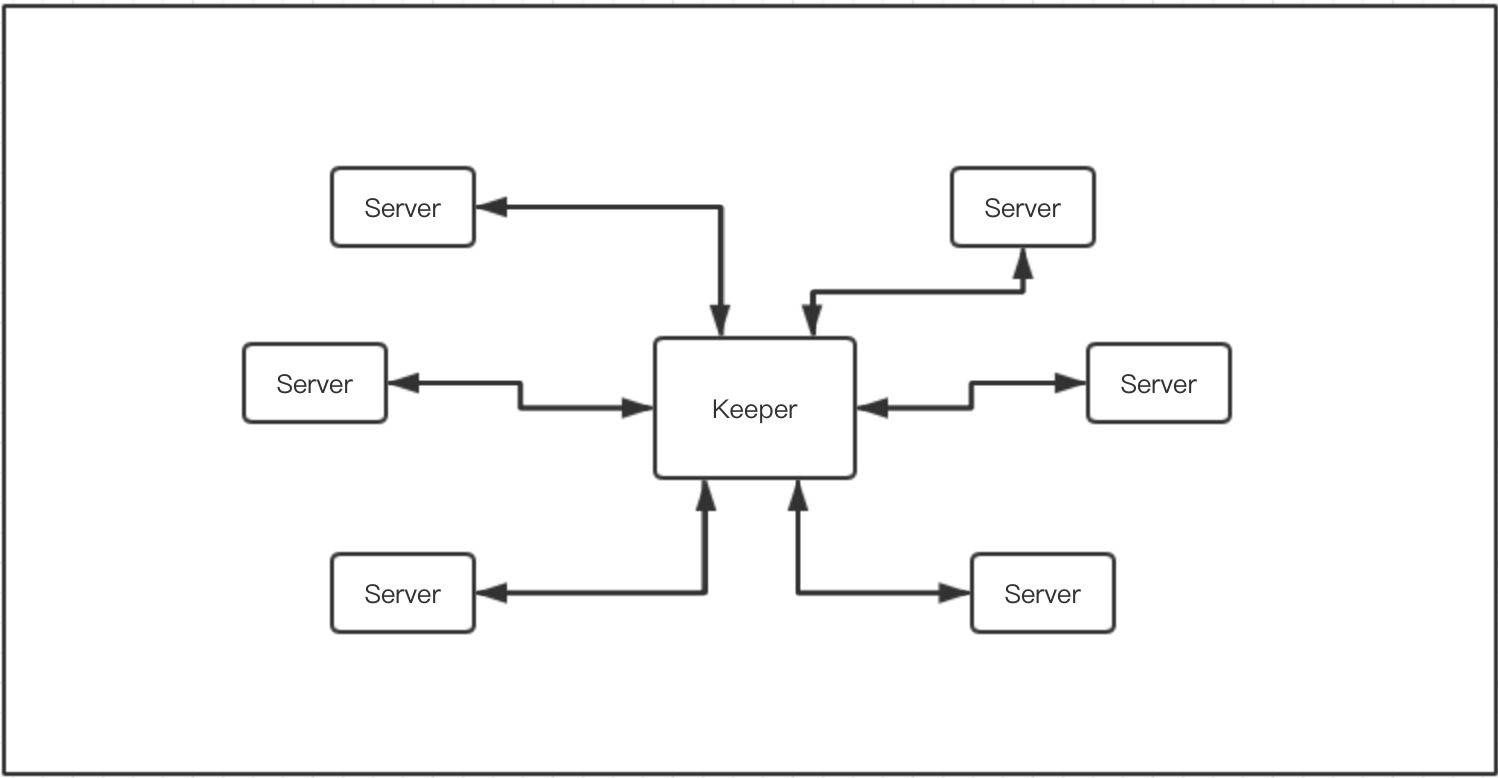
\includegraphics[scale=0.3]{share.png}
			\end{center}
			\paragraph{Section 2: The Element Catalog}
			\subparagraph{Elements and their properties}
			\begin{itemize}
			\item{Keeper} The keeper is a data storage center which holds the shared data.
			\item{Server} The server is an entity which stores and fetches data from the Keeper. For example, when a customer temporarily terminates the process, server should save the context for a future reference.
			\end{itemize}
			\subparagraph{Relations and their properties}
			During the fetching process, there may not exist the record, so there should be an exception. Also, in the saving process, to those records that already existed, saving process should be an update to the old version.
			\subparagraph{Element interfaces}
			The Keeper should provide the find and insert interfaces to the servers.
			\subparagraph{Element behavior}
			The servers save and fetch the data from the Keeper.
			\paragraph{Section 3: Context Diagram}
			\begin{center}
			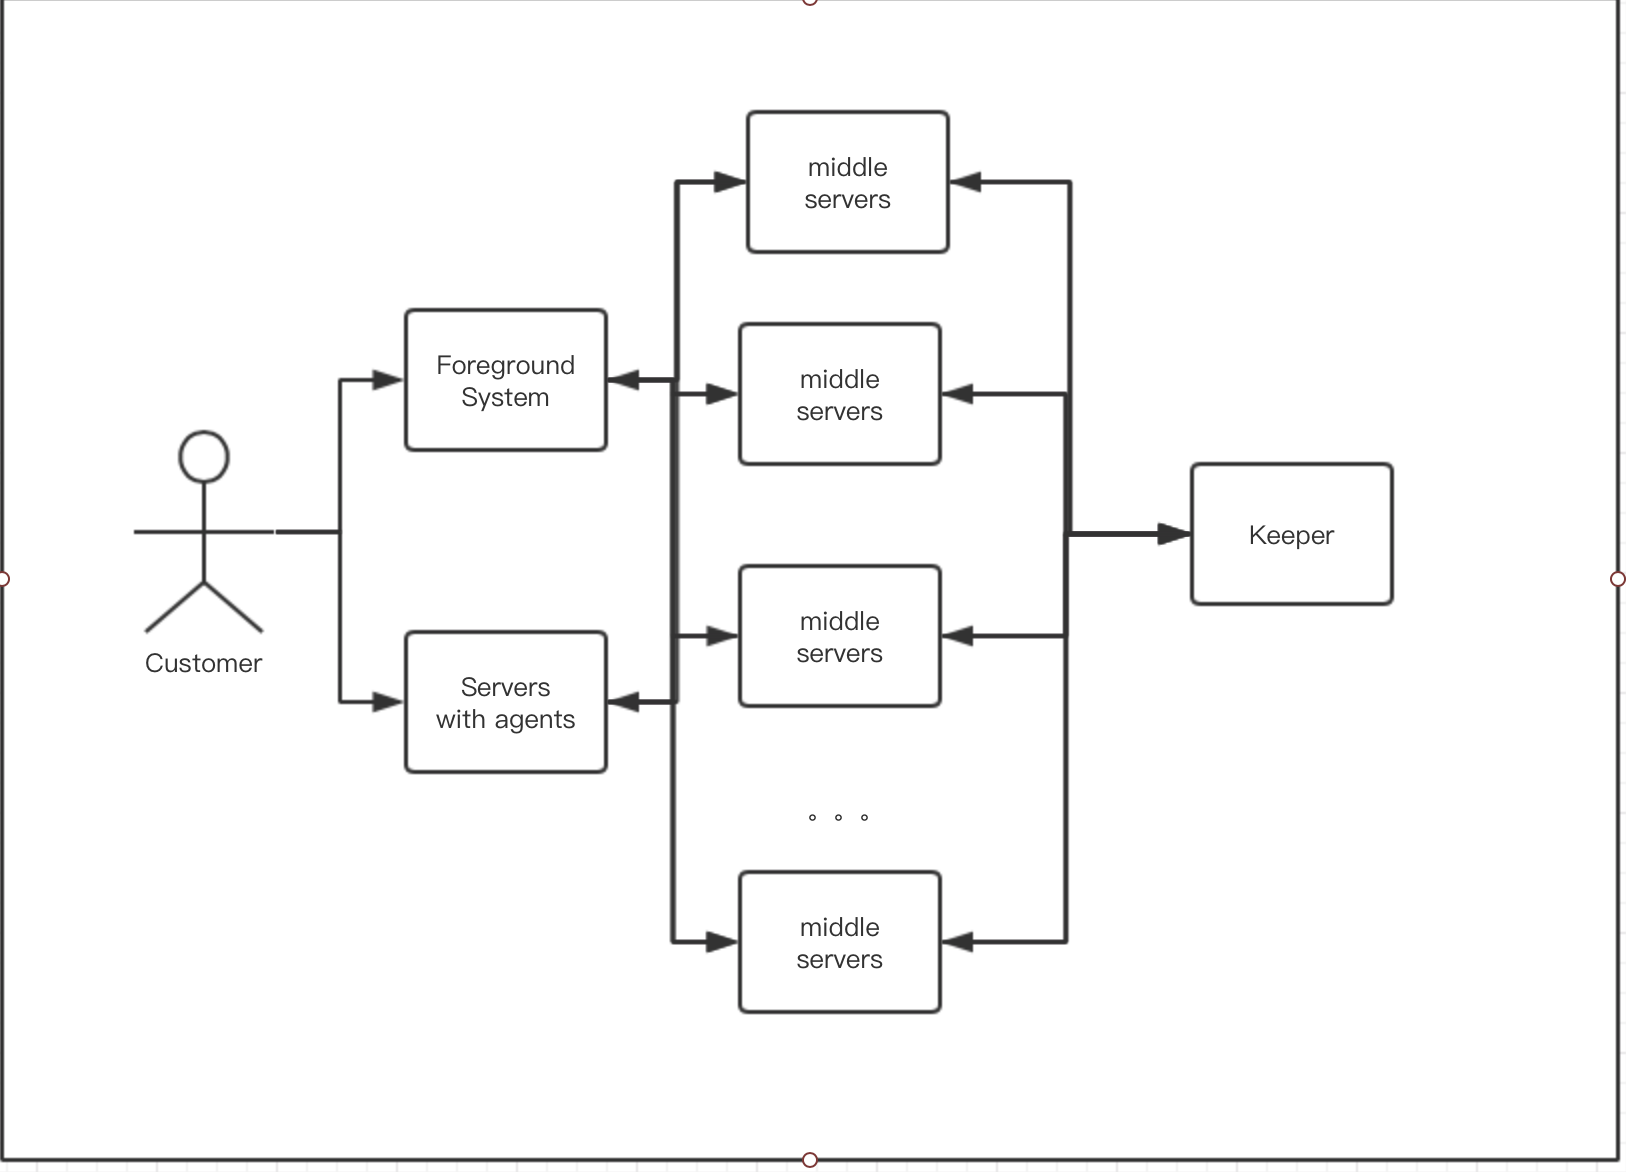
\includegraphics[scale=0.3]{share2.png}
			\end{center}
			\paragraph{Section 4: Variability Guide}
			Because the data storage is not the only responsibility keeper takes, so in the future, it may be  divided into several more specific components, that is to say, the keeper in this view may be changed to a data repository or other data center.
			\paragraph{Section 5: Rationale}
			The design problem came from the requirement "A customer can be interrupted (for technical reasons, for example) or suspended by the customer or the representative ... In any case, C4 has to manage the context that persists and can be recalled."
			In order to do this, there should be a mechanism that stores and fetches the context. There are several options. For example, we can save the information in the agent's PC, or save in the DB provided by the third party. But both of them are infeasible. There is no persistent data caching on the agent workstations, and DB may not be changed since it is provided by the third party. So finally, we choose to save the information in the Keeper, as it is also used to synchronize the event and resolve the conflict as mentioned in the sections before.

		\subsubsection{Decomposition View} 
			\paragraph{Section 1: The Primary Presentation}
			\begin{center}
			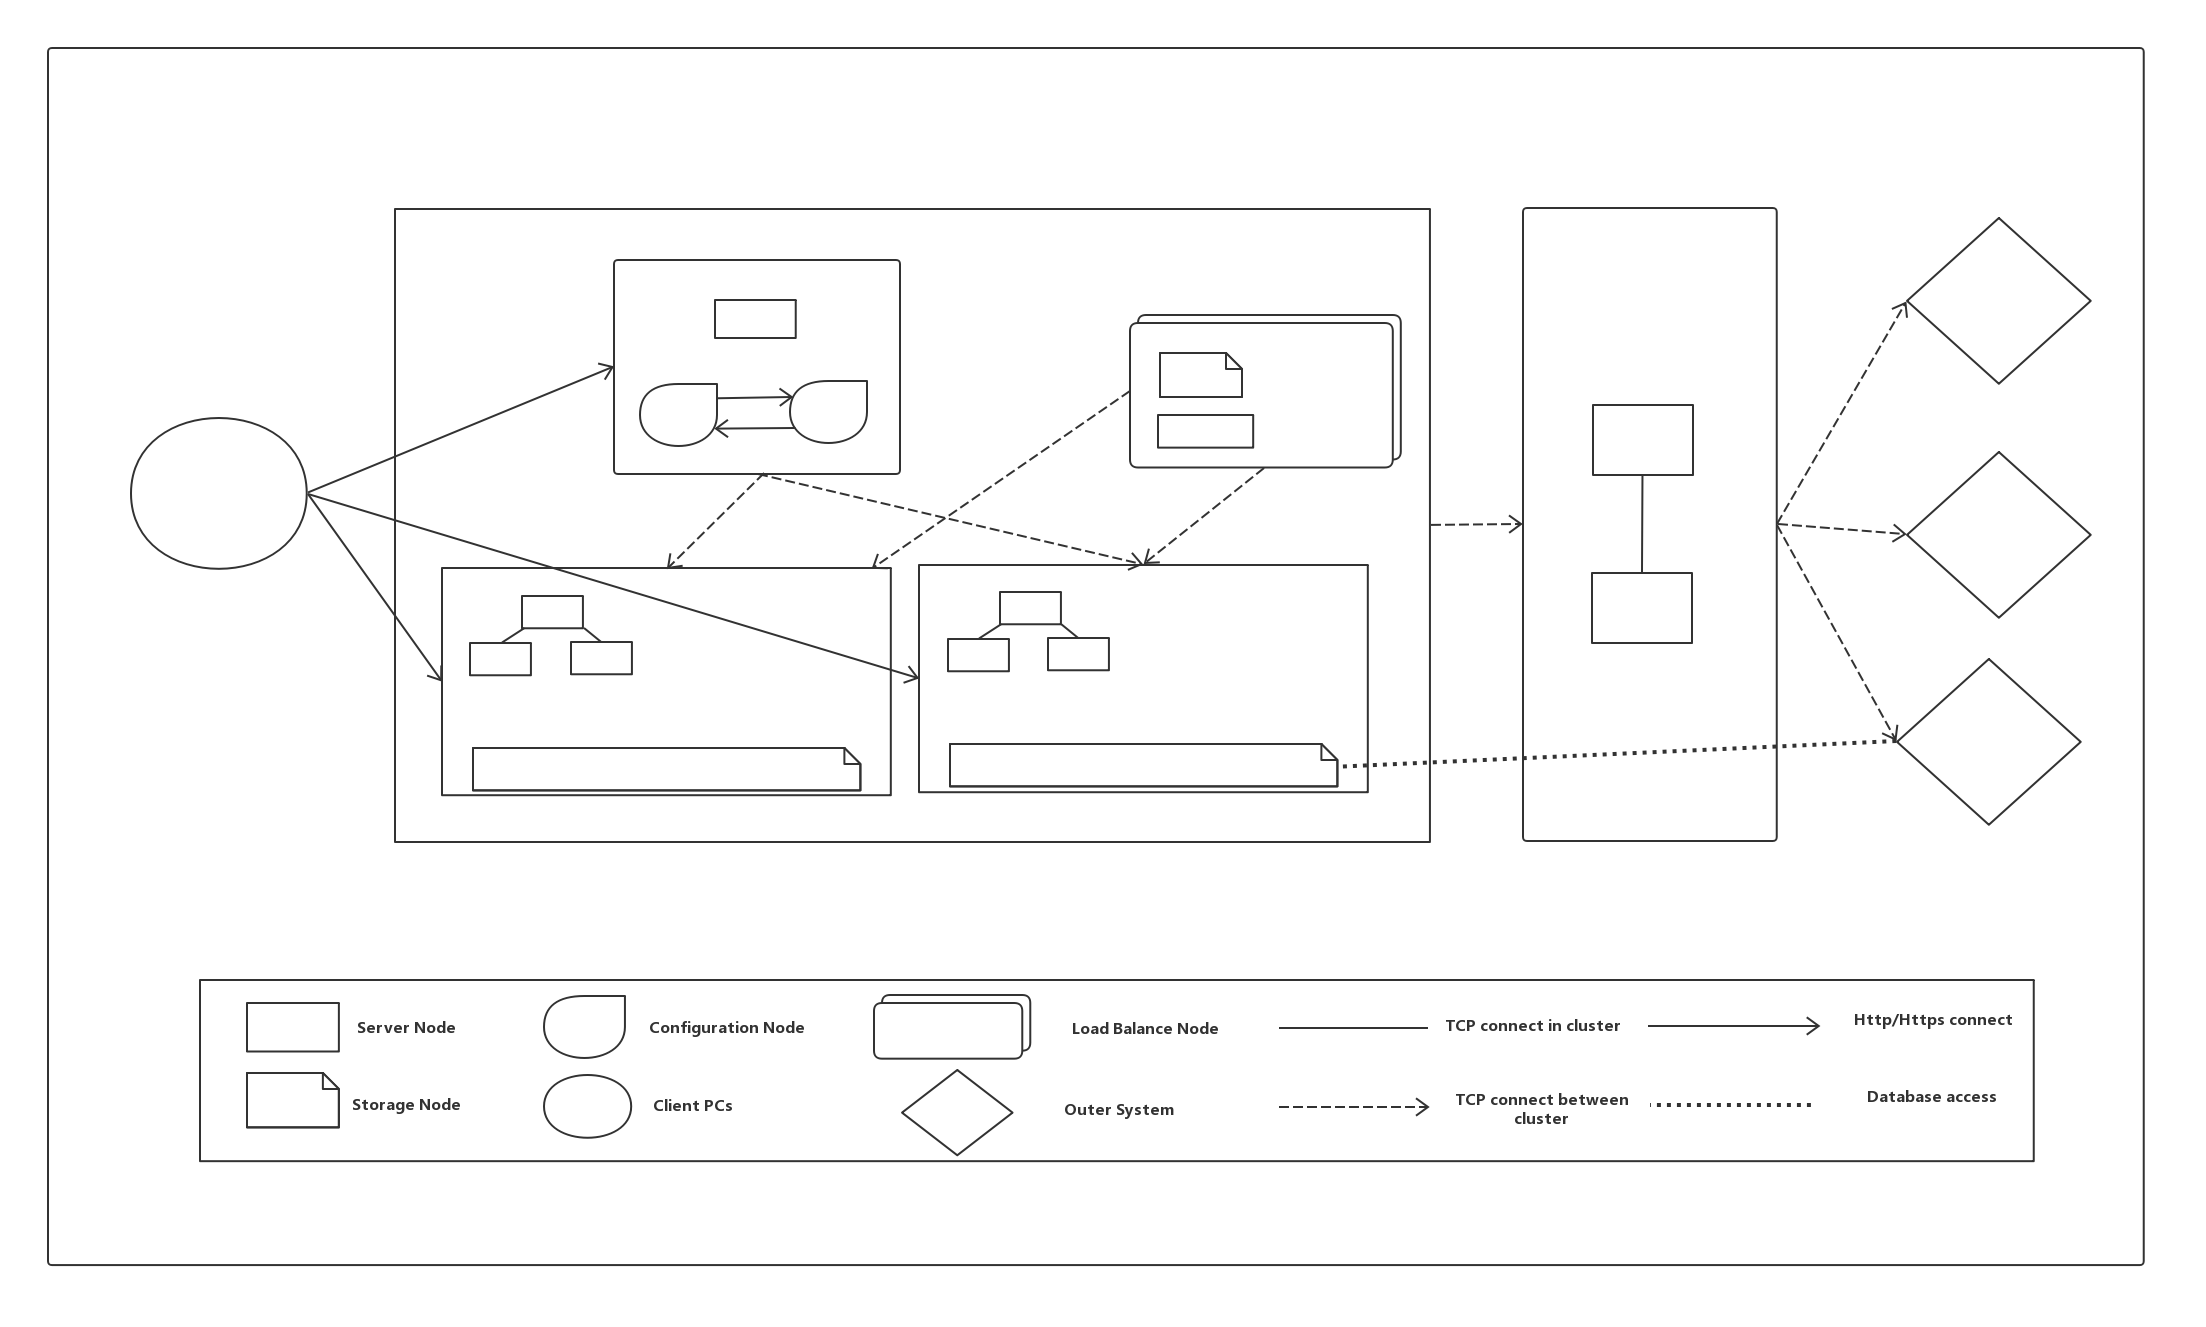
\includegraphics[scale=0.15]{decom_section1.png}
			\end{center}
			\paragraph{Section 2: The Element Catalog}
			The C4 system is consisted of these important sub-module to decompose:  master node , normal server node , storage node , configuration node , load balance node. To resolve the normal phone request (contains the sync-request and async-request) , the normal server nodes are responsible to tackle the service from customers. Moreover , the storage nodes have to save the current session , cache the query on DB , and other cache to the locks . Load balance node has to detect the load in the whole system , and reschedule the load accordingly. 
			\paragraph{Section 3: Context Diagram}
			\begin{center}
			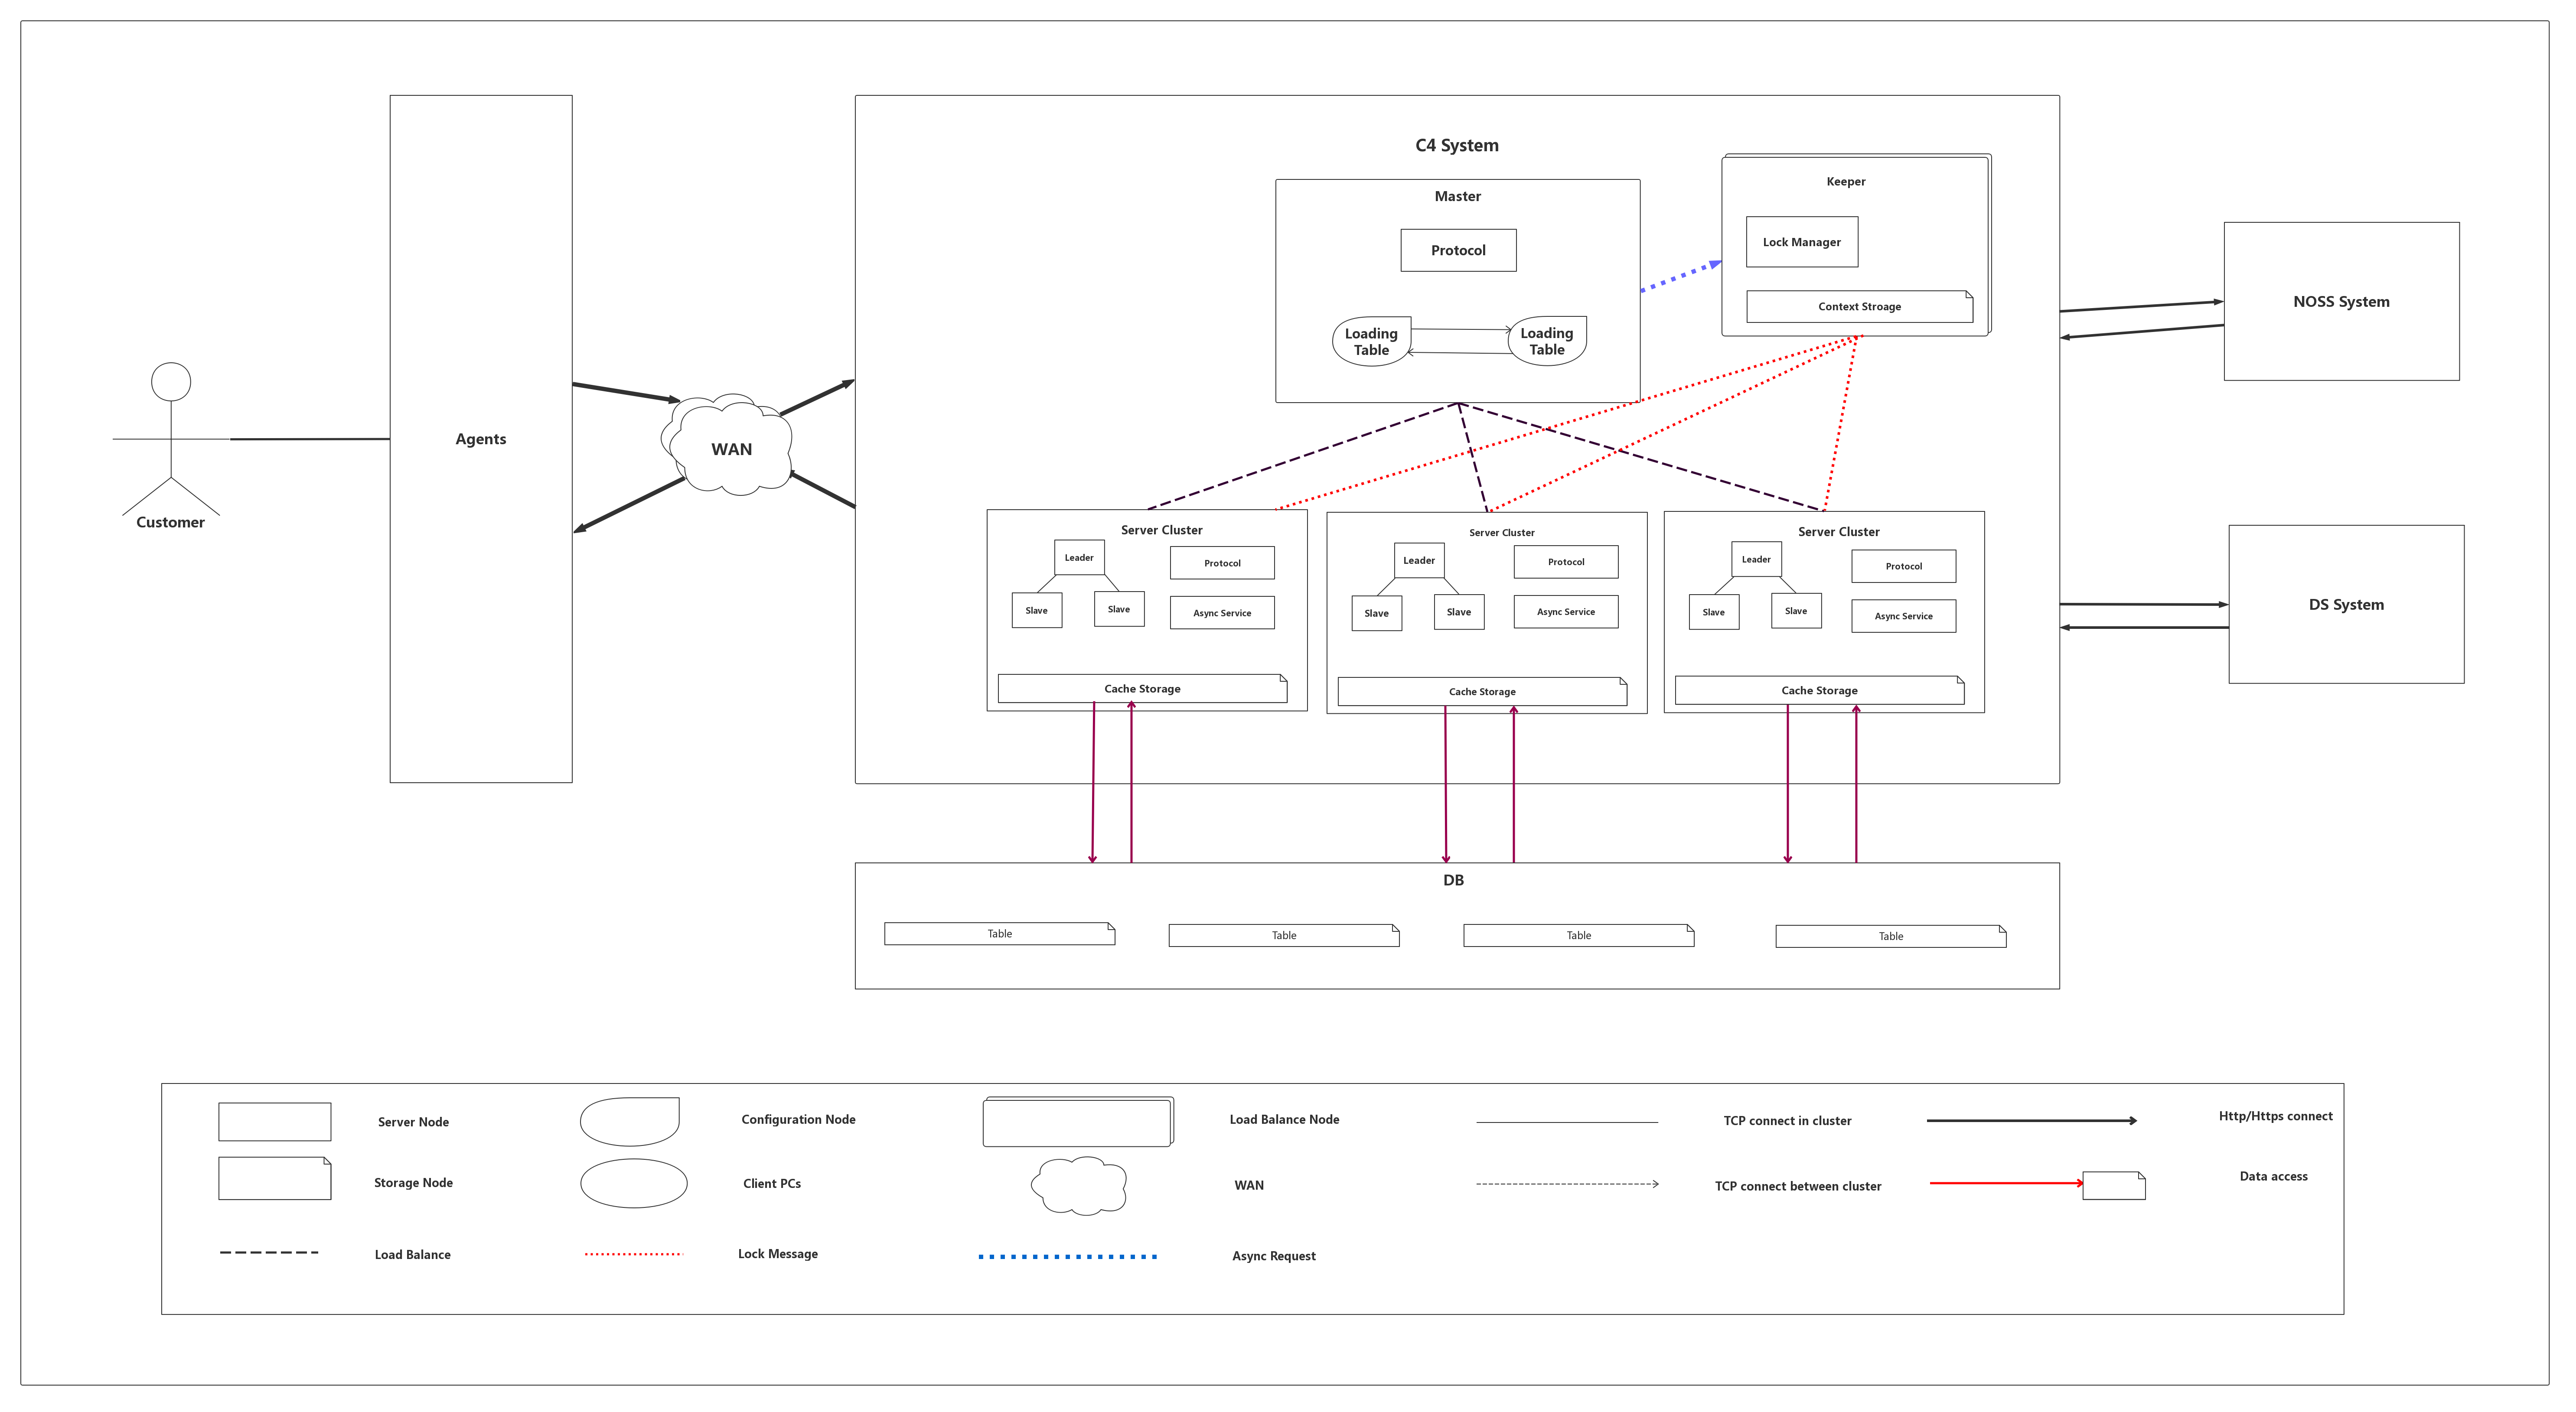
\includegraphics[scale=0.05]{decom_section2.png}
			\end{center}
			\paragraph{Section 4: Variability Guide}
			The decomposition view represents the template module in the C4 system , and to exercise the variation points , you are recommended to run the server node. With the sync-request (like fetching user basic information , setting up a new session)  and async-request (conflict between the different sessions) , you could catch the key points in the master.
			\paragraph{Section 5: Rationale}
			The PC agents communicate with C4 system across the WAN. 
			Master node stands for the whole manager of C4 system . That is ,  the master node uses the loading table to temporarily record the load status of all subordinate slave server clusters, and can timely alarm and resource reallocation. The master node also contains a protocol subnode, which is mainly used to help the master node process user requests. After the agents send the request, they will first be parsed by the master node to inform the agents of the required service node location, and then the agents will send the request to the target server.	
			The keeper is responsible for asynchronous event processing and session saving between server nodes. Use Lock Manager to allocate locks and save contexts through context storage.
			The server node is mainly responsible for periodically reporting heart beat status to the master node, and can perform hot backup between nodes. Please note that one server node here is also a cluster. In our design, one cluster is responsible for a certain range. The service (similar to the microservices architecture), and the leader is elected by the vote inside the cluster to perform resource scheduling and service allocation to the subordinate slave. In addition, the server node also supports the processing of the protocol and async service. Responsible for the interaction of the NOSS and DS systems. The cache storage is responsible for the caching of the external DB system. Since each business request will design a query of more than a dozen data tables, considering the time loss of the cascaded query, we use the cache mechanism to The query result is cached inside the server.
			
	\subsection{Mapping Between Views}
	TODO

	\subsection{Rationale}
	Explain what decision we have made in our views.

	\subsection{Directory}


	\section{Personal Remarks}
	\subsection{Statement of ...}
	\subsection{Statement of ...}
	\subsection{Statement of ...}
	\subsection{Statement of ...}
\end{document}